\documentclass[]{paper}

\usepackage{listings}
\usepackage{url}
\usepackage[autostyle]{csquotes}  
\usepackage{graphicx}


\begin{document}


\title{Visualizing network traffic in a distributed software system}
\author{Nico Westerbeck}
\date{\today}
\maketitle{}
\tableofcontents

\section{Introduction}

In this paper we explain and demonstrate a way how to visualize network flow in a distributed software system, making it easier to solve placement issues when scaling an application. For this we will first discuss the characteristics of a distributed software system and common fallacies, then discuss how data visualization can solve those problems and in the end present and discuss our solution.

\section{Distributed systems}

First we need to define what a distributed system is, for this see the definition by \cite{Tanenbaum}
\begin{displayquote}
A distributed system is a collection of independent computers that
appears to its users as a single coherent system.
\end{displayquote}
This means the underlying system will take care of any issues of distribution and present the user with an interface as if he was working with a single machine. The reason to distribute a system is to scale beyond the limits of one machine, as computation power, memory and other resources are limited when working on one node. To still be able to incorporate big amounts of data or request, a system has to distribute across several connected machines, dividing the load on those machines. To coordinate all those machines, a certain communication overhead is imminent. Data needs to be passed around as it is not possible to hold it in RAM or on disks on every machine. 

In HPC distributed frameworks such as MPI \cite{MPI} provide measures to distribute an appplication on a cluster. MPI facilitates this communication by providing C-routines for spreading or collecting data in the cluster. In software- and webdevelopment, the microservice architecture \cite{martinfowler2014microservices} splits a typical software system into independent units which can run on independent machines, being connected by APIs. The communication is thus managed by the software design process.

In both cases, communication is a central matter of concern, as it can easily become a bottleneck. Thus we propose to utilize data visualization to make the topic more accessible.

\section{Network traffic}
Netework traffic in an IP based system happens in packets. Those packets have a sender and a receiver and will carry a payload of data to that receiver. Usually those packets are transmitted via cable or wireless transmission over a certain distance, sender and receiver are physically separate units. This channel imposes certain limitations on the communication such as limited bandwidth, packet loss, latency or transmission errors. The latter is usually dealt with at a transport level and thus not addressed here. Packet loss can be avoided or reduced by using TCP and thus is also out of the scope of this paper. Latency and bandwidth however are unavoidable problems. Depending on the type of application, typically either of the two is the limiting factor, and the software engineer has to take those into account when developing the application. 

Data visualization can be used to aid the developer in this process by reflecting the network structure visually and displaying the parameters in a visual way, allowing tweaking of parameters to determine a good setup for the respective application. Also, changes of the network structure should be in the scope of the application, as this might also be in the scope of control of the engineer and he might want to set up the network in a way most beneficial for the application. The parameters of bandwidth and latency can be displayed in various scales. Latency could be associated with the distance between two nodes, which however leaves a placement problem as it might not be possible to arrange all nodes in a way that respects those distances. Also latency could be associated with some kind of movement speed, as the process of transferring a packet resembles the characteristics of a physical movement. Bandwidth could be associated with the with of a band between two nodes, as the name suggests. Also color intensity or node size might serve as a good representation. In all of this it would be important that the developer gets instant visual feedback on parameter changes, as otherwise it would be possible to conduct real world tests in a physical setup of the system instead to get more accurate results.

\section{Our solution}

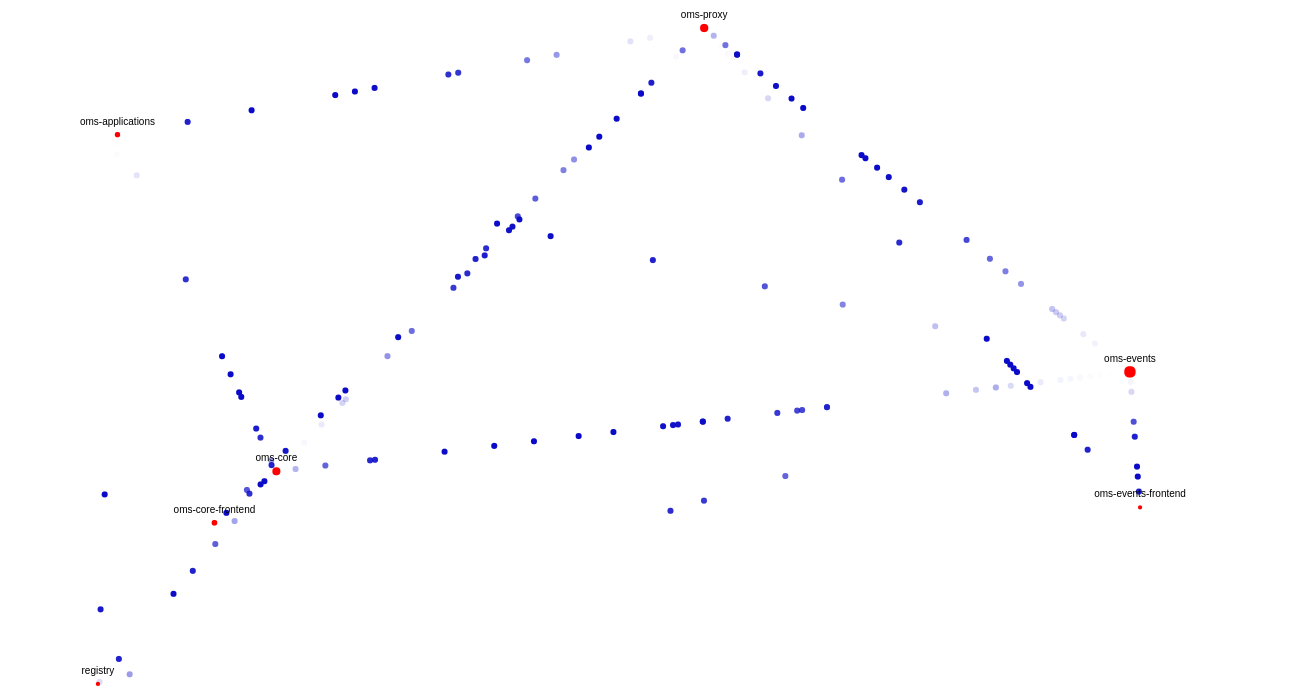
\includegraphics[width=11cm]{screenshot.png}

We decided to focus our visualization solution on those parameters as discussed in previous section. We decided to display the nodes by placing circles on a 2D canvas. The size of the circle is determined by the total volume of incoming and outgoing data at the node, indicating the load of that node. This way the developer can decide to replicate a node in case it gets too loaded. For this, the GUI offers an easy duplicate function, which copies all values of a node to an exact copy of that node. For more intuitive reading, the user can assign a name to each of the circles and also store the IP, a necessary parameter for routing, in the node. Also he can arrange the nodes freely on the 2D space, based on how it is most intuitive.

We decided to display network traffic by visualizing each packet by a blue boid, flying from its source to its destination. The speed of these boids is determined by the latency of the connection, while the amount of boids spawned is dependant on the data volume transferred across that connection. This way, the eye perceives a different color intensity based on how many boids are flying between two nodes. To support that effect, we added a slight trail to each node. Also, the speed of the boids flying is perceived easily and gives an intuitive hint on the latency between two nodes. The developer can easily spot slow moving or dark blue trails as lines of high congestion and try to fix these issues by replicating nodes or improving the situation of the underlying network connection.

To facilitate all these, we offer an intuitive GUI with a modern look, that makes it easy to adjust parameters and set up the network in the way that is.

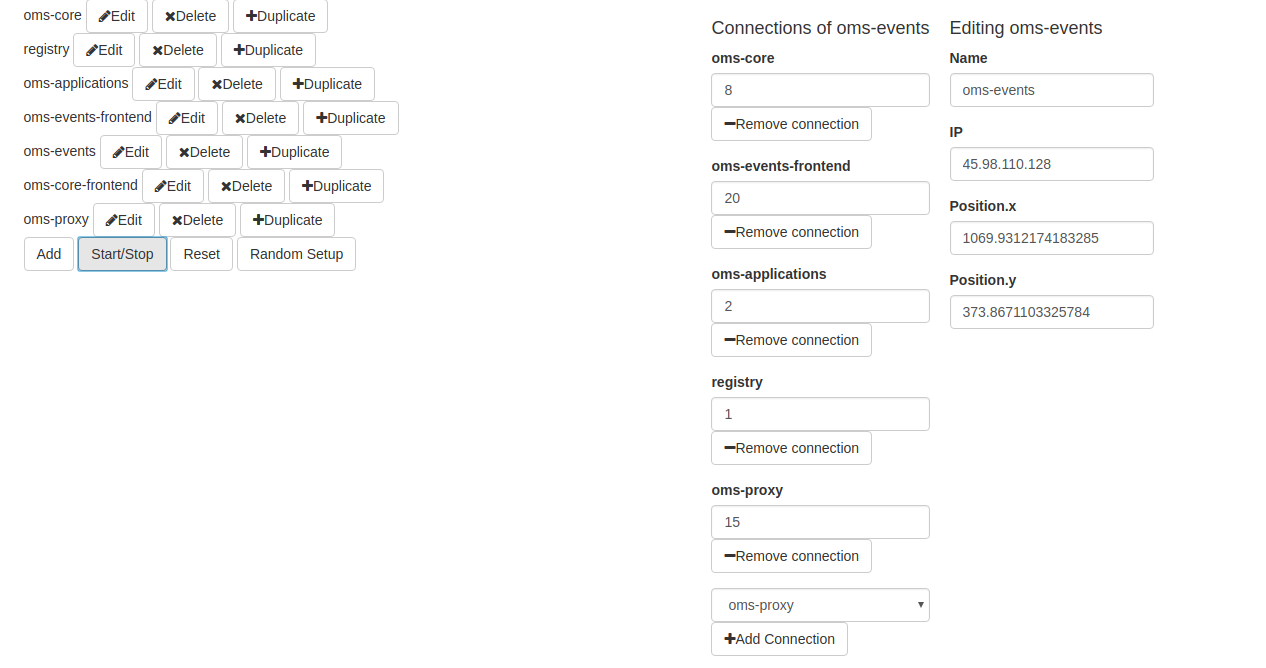
\includegraphics[width=11cm]{screenshot2.png}

\section{Discussion}

We evaluated our system to represent the distributed architecture of the OMS \cite{OMS}, a membership management system developed by the NGO AEGEE. We found our solution perfectly capable to represent the architecture and connections, but manually creating all connections posed a burden which limits the usability of our system. Thus we researched possibilities to automatically reflect a structure without the developer interferring and found a solution to monitor a docker-based architecture by injecting tcpdump packet captures into each container, forwarding those captured packets to an analyzing monitor which then sets the parameters in the visualization solution. However, this is limited to docker-based architectures only and to not loose generality we decided to not implement this feature. It can be added in case this used in a real world scenario though.

Also we noted a performance drop when visualizing large amounts of nodes. To overcome this, we could add an alternative visualisation which uses bands between the nodes in different widths and colors to visualize the network traffic. The solution as it is however is suited to visualize small to medium size problems. A large-scale visualisation would require the automated data-capturing and analyzing as the effort to manually add all nodes increases by size.
\bibliographystyle{unsrt}
\bibliography{paper}

\end{document}